\documentclass[10pt,a4paper]{beamer}
				
\usepackage[ngerman]{babel}
\usepackage[T1]{fontenc}
\usepackage[utf8]{inputenc}
\usepackage{varioref}
\usepackage{hyperref}
\usepackage{cleveref}
\usepackage{amsmath}
\usepackage{amsfonts}
\usepackage{amssymb}
\usepackage{makeidx}
\usepackage{graphicx}
\usepackage{csquotes}

\setbeamercolor{logo}{bg=white}  %controls the color of the logo area
\setbeamertemplate{navigation symbols}{}

\usetheme{PaloAlto}
\renewcommand{\footnotesize}{\small}
\newcommand{\pftn}[1]{\let\thefootnote\relax\footnotetext{\tiny #1}}
\newcommand{\ftn}[2]{\footnote[#1]{\tiny #2}}

\logo{
\includegraphics[width=0.155\linewidth]{hbbk-logo}}
\author{Luca Hülsmann \and Luca Kiebel \and Luca Hartmann}
\title{Islamischer Staat}
\date{\today}
\setlength{\itemsep}{10pt}
\begin{document}
\begin{frame}
\titlepage
\end{frame}

\begin{frame}
\frametitle{Inhaltsverzeichnis}\tableofcontents
\end{frame}

\section{Einleitung}
\begin{frame}
\frametitle{Einleitung}
\framesubtitle{Was ist der Islamische Staat?}
Beim \enquote{Islamischen Staat} handelt es sich um eine islamistische Terrororganisation, deren Mitglieder sich zu einer radikalen Auslegung des sunnitischen Islam bekennen. Der Islamische Staat kontrolliert zur Zeit Teile Syriens und des Iraks. Hier hat die Organisation am 29. Juni 2014 ein Kalifat ausgerufen. Zur Zahl der IS-Kämpfer gibt es nur Schätzungen, die von einigen zehntausend bis zu mehreren hunderttausend reichen.\pftn{https://www.lpb-bw.de/islamischer-staat.html}
\end{frame}

\section{Geschichte}
%%%%%%%%%%%%%%%%%%%%%%%%%%%%%%%%%%
% HÜSLMANN
%%%%%%%%%%%%%%%%%%%%%%%%%%%%%%%%%%



%Anführer
\section{Wichtige Personen}
\subsection{Anführer des IS}
\begin{frame}
\frametitle{Anführer des IS}
\framesubtitle{Wie viele gab und gibt es noch?}
\begin{itemize}
	\item Abū Mus'ab az-Zarqāwī
\end{itemize}
\end{frame}

\begin{frame}
\frametitle{Anführer des IS}
\framesubtitle{Abū Mus'ab az-Zarqāwī}
\begin{itemize}
	\item Geboren 30. Oktober 1966 in Jordanien; Gestorben 7. Juni 2006 im Irak \pause
	\item Mitglied der Terrororganisation al-Qaida im Irak und Gründer des IS
	\pause
	\item Gestorben durch einen gezielten Luftanschlag
\pftn{https://de.wikipedia.org/wiki/Abū\_Musab\_az-Zarqāwī}
\end{itemize}
\end{frame}

\begin{frame}
\frametitle{Anführer des IS}
\framesubtitle{Wie viele gab und gibt es noch?}
\begin{itemize}
	\item Abū Mus'ab az-Zarqāwī
	\item Abu Abdallah ar-Raschid al-Baghdadi
\end{itemize}
\end{frame}

\begin{frame}
\frametitle{Anführer des IS}
\framesubtitle{Abu Abdallah ar-Raschid al-Baghdadi}
\begin{itemize}
	\item Ein \enquote{schattenhaftes Pseudonym}
	\pause
	\item Anführer von 2006 - 2010
	\pause
	\item Getötet durch einen Sturmtrupp
\pftn{https://de.wikipedia.org/wiki/Abu\_Abdallah\_ar-Raschid\_al-Baghdadi}
\end{itemize}
\end{frame}

\begin{frame}
\frametitle{Anführer des IS}
\framesubtitle{Wie viele gab und gibt es noch?}
\begin{itemize}
	\item Abu Mus'ab az-Zarqāwī
	\item Abu Abdallah ar-Raschid al-Baghdadi
	\item Abu Bakr al-Baghdadi
\end{itemize}
\end{frame}

\begin{frame}
\frametitle{Anführer des IS}
\framesubtitle{Abu Bakr al-Baghdadi}
\begin{itemize}
\item Geboren am 1. Juli 1971 im Irak
\pause
\item Anführer seit 2010 mit einem Kopfgeld von 25 Millionen US-Dollar
\pause
\item Lebensstatus unbekannt
\pftn{https://de.wikipedia.org/wiki/Abu\_Bakr\_al-Baghdadi}
\end{itemize}
\end{frame}

%%%%%%%%%%%%%%%%%%%%%%%%%%%%%%%%%%%%%%%%%
% Aktuell Kontrollierte Gebiete
%%%%%%%%%%%%%%%%%%%%%%%%%%%%%%%%%%%%%%%%%

\section{Aktuell kontrollierte Gebiete}


%Struktur
\section{Struktur im IS}
\begin{frame}
\frametitle{Struktur im IS}
\framesubtitle{Aufbau des IS}
\begin{center}
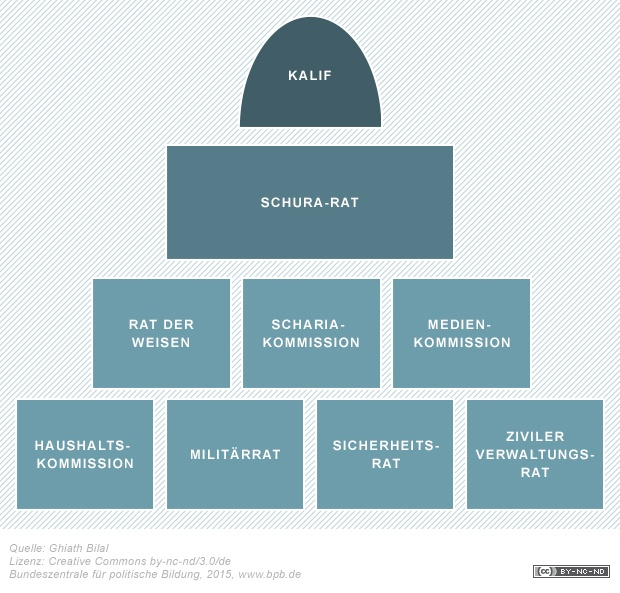
\includegraphics[width=0.7\linewidth]{struktur}
\end{center}
\end{frame}

\begin{frame}
\frametitle{Aufbau des IS}
\framesubtitle{Der Kalif}
\begin{itemize}
	\item Anführer des IS
	\pause
	\item Leiter des Schura-Rats
	\pause
	\item Verteilung der einzelnen Leiter Rollen der Gremien
\end{itemize}
\pftn{https://www.bpb.de/politik/extremismus/islamismus/202373/der-islamische-staat-interne-struktur-und-strategie?p=all}
\end{frame}

\begin{frame}
\frametitle{Aufbau des IS}
\framesubtitle{Der Schura-Rat}
\begin{itemize}
	\item Zuständig für die Beratung des Kalifen
	\pause
	\item Veto Recht den Kalifen neu zu wählen
	\pause
	\item Überwachung der Gremien
\pftn{https://www.bpb.de/politik/extremismus/islamismus/202373/der-islamische-staat-interne-struktur-und-strategie?p=all}
\end{itemize}
\end{frame}

\begin{frame}
\frametitle{Aufbau des IS}
\framesubtitle{Rat der Weisen}
\begin{itemize}
	\item Zuständig für die Kommunikation zwischen dem IS und der Bevölkerung
	\pause
	\item Verantwortlich für die Anerkennung des IS
\pftn{https://www.bpb.de/politik/extremismus/islamismus/202373/der-islamische-staat-interne-struktur-und-strategie?p=all}
\end{itemize}
\end{frame}

\begin{frame}
\frametitle{Aufbau des IS}
\framesubtitle{Scharia-Kommission}
\begin{itemize}
	\item Fungiert als Obergericht in wichtigen Konflikten
	\pause
	\item Zuständig für die Überwachung des medialen Bereichs
\pftn{https://www.bpb.de/politik/extremismus/islamismus/202373/der-islamische-staat-interne-struktur-und-strategie?p=all}
\end{itemize}
\end{frame}

\begin{frame}
\frametitle{Aufbau des IS}
\framesubtitle{Medien-Komission}
\begin{itemize}
	\item Zuständig für die externe mediale Kommunikation
	\pause
	\item Veröffentlichung der Propaganda
\pftn{https://www.bpb.de/politik/extremismus/islamismus/202373/der-islamische-staat-interne-struktur-und-strategie?p=all}
\end{itemize}
\end{frame}

\begin{frame}
\frametitle{Aufbau des IS}
\framesubtitle{Haushalts-Kommission}
\begin{itemize}
	\item Verantwortlich für die Geldquellen des IS
	\pause
	\item Überwacht die Ausgaben des IS
\pftn{https://www.bpb.de/politik/extremismus/islamismus/202373/der-islamische-staat-interne-struktur-und-strategie?p=all}
\end{itemize}
\end{frame}

\begin{frame}
\frametitle{Aufbau des IS}
\framesubtitle{Militärrat}
\begin{itemize}
	\item Zuständig für Militärisches darunter zählt:
	\pause
	\item Strategische Planung sowie Planung der Attentate
	\pause
	\item Waffenproduktion sowie Kriegsführung
\pftn{https://www.bpb.de/politik/extremismus/islamismus/202373/der-islamische-staat-interne-struktur-und-strategie?p=all}
\end{itemize}
\end{frame}

\begin{frame}
\frametitle{Aufbau des IS}
\framesubtitle{Sicherheitsrat}
\begin{itemize}
	\item Sorgt für den Schutz des Kalifen sowie vor Infiltration des IS
	\pause
	\item Handlungsbeobachtung der Führungsebene
	\pause
	\item Spezialeinheit für gezielte Mordanschläge und Entführungen
\pftn{https://www.bpb.de/politik/extremismus/islamismus/202373/der-islamische-staat-interne-struktur-und-strategie?p=all}
\end{itemize}
\end{frame}

\begin{frame}
\frametitle{Aufbau des IS}
\framesubtitle{Ziviler Verwaltungsrat}
\begin{itemize}
	\item Verantwortlich für die Verwaltung
	\pause
	\item D.h. Dokumentation von Veranstaltungen
	\pause
	\item Preiskontrolle der Nahrungsmittel
\pftn{https://www.bpb.de/politik/extremismus/islamismus/202373/der-islamische-staat-interne-struktur-und-strategie?p=all}
\end{itemize}
\end{frame}

\begin{frame}
\frametitle{Aufbau des IS}
\framesubtitle{Verdienst im IS}
Internationale Quellen sind sich uneinig, wie hoch der tatsächliche Soll ist, aber Schätzungen liegen im Bereich von \$50 bis \$800 
\pftn{https://www.theguardian.com/world/2016/jan/20/islamic-state-to-halve-fighters-salaries-as-cost-of-waging-terror-starts-to-bite}
\pftn{http://www.ibtimes.co.uk/payslip-reveals-how-isis-fighter-earns-only-50-month-gets-sex-slave-bonus-1556690}
\end{frame}


% Einfluss der restlichen Welt
\section{Einfluss der westlichen Welt}
\subsection{Entstehung des IS}
\begin{frame}
\frametitle{Einfluss der westlichen Welt}
\framesubtitle{Entstehung des Islamischen Staates}
\begin{itemize}
\item Der IS ist \enquote{made-in-the-USA}
\pause
\item USA unterstützen oft Terroristen
\pause
\item Besetzung des Irak sorgte für Arbeitslosigkeit
\end{itemize}
\pftn{https://www.globalresearch.ca/america-created-al-qaeda-and-the-isis-terror-group/5402881}
\end{frame}

\subsection{Wachsen des IS}
\begin{frame}
\frametitle{Einfluss der westlichen Welt}
\framesubtitle{Wachsen des Islamischen Staates}
\begin{itemize}
\item \enquote{Hilfe} bei der Destabilisierung des Syrischen Regimes\ftn{1}{https://www.n-tv.de/15177536}
\pause
\item Auflösung von Gefängnissen im Irak liefert Soldaten\ftn{2}{ https://www.theatlantic.com/international/archive/2015/10/how-isis-started-syria-iraq/412042/}
\end{itemize}
\end{frame}

\begin{frame}
\frametitle{Einfluss der westlichen Welt}
\framesubtitle{Wachsen des Islamischen Staates}
\begin{itemize}
\item Völliges Versagen der politischen Ordnung\ftn{3}{http://www.deutschlandfunkkultur.de/ursachen-des-is-terrors-die-verantwortung-des-westens.1270.de.html?article=321197}
\pause  
\item US-Außenminister John Kerry: \enquote{Wir haben den IS wachsen lassen}\ftn{4}{https://wikileaks.com/podesta-emails/emailid/357}
\end{itemize}
\end{frame}





\begin{frame}
\titlepage
\end{frame}

\end{document}